\chapter{Testing and comparing models for RoboTour}
\label{chapter:testingandcomparing}

The RoboTour 2019 competition took place in Deggendorf, Germany. It was our first
opportunity to train and test several segmentation models. In this chapter, we introduce
our datasets, the way we preprocess and augment data before feeding it to ConvNet and
present the HSV baseline model.
We also compare several models we tested before the competition and report results.

\section{Datasets}
\label{sec:datasets}

The first dataset that has already been published in \cite{bib:suppajariabka2017}
contains~\textbf{333} labeled pictures in 4:3 ratio taken in the city park of
\textit{Lednice}. See Figure \ref{img:lednice_examples} for examples from this dataset.

\begin{figure}[!h]
	\begin{center}
	    \subfloat[]{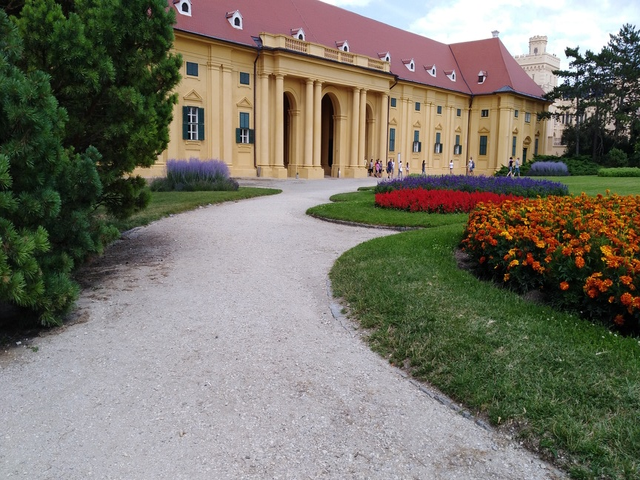
\includegraphics[width=0.48\textwidth]{images/lednice_example1.png}}
		\quad
		\subfloat[]{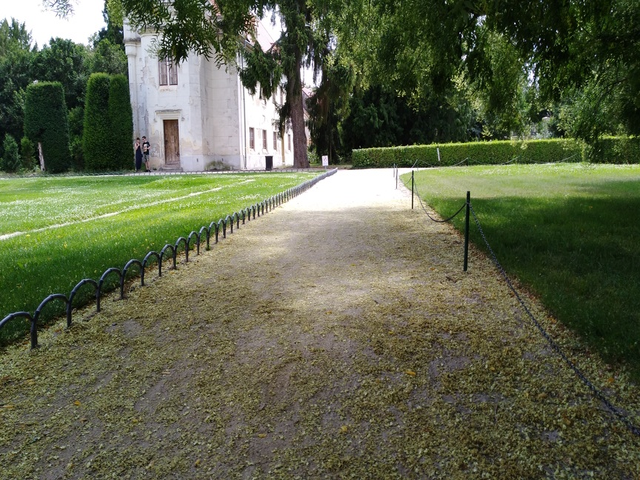
\includegraphics[width=0.48\textwidth]{images/lednice_example2.png}}
	\end{center}
	\caption[Examples from the city park of Lednice]{Examples from the city park of Lednice.}
	\label{img:lednice_examples}
\end{figure}

Since the latest contest took place in Deggendorf, we wanted to create a new dataset
capturing the park which surrounds \textit{Deggendorf Institute of Technology}.
Images were captured by
Android Huawei phone in 4:3 ratio catching various weather conditions, which prevented models
overfit to specific conditions.
One can find there are various types of pavements, wet and dry roads, sun shining right to the
camera lens, people walking or riding a bicycle, bridges, benches, shadows and leaves on
the roads, river, grass, flowers, gravel and railway. Examples are shown in Figure
\ref{img:deggendorf_examples}.

Testing one day before the competition
revealed that the dataset was quite imbalanced because all of the images contained driveable
path. Models had always searched for some sort of road, which resulted in very bad
predictions of images containing mostly grass or non-driveable segments. Therefore, we let
the robot capture additional pictures with grass covering huge part of images.
See predictions before and after the dataset has been extended in Figure
\ref{img:beforeafterextending}. We picked 61 and manually labeled them.
The Deggendorf dataset now contains \textbf{344} images in total.

\begin{figure}[!h]
	\begin{center}
	    \subfloat[]{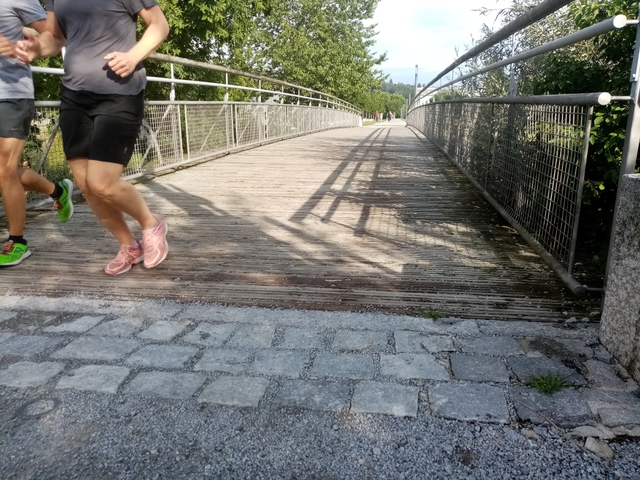
\includegraphics[width=0.48\textwidth]{images/deggendorf_example1.png}}
		\quad
		\subfloat[]{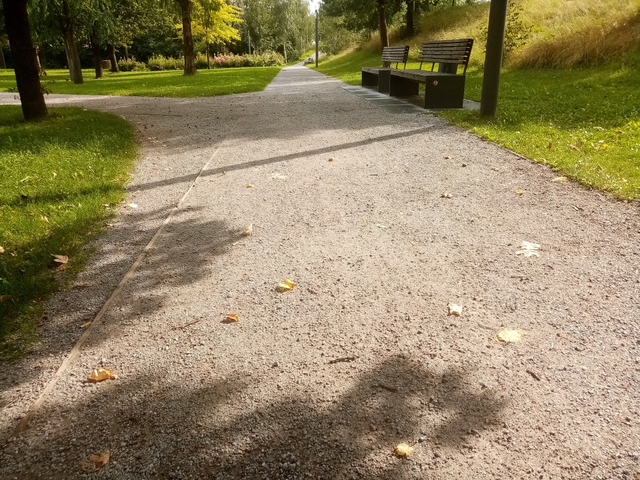
\includegraphics[width=0.48\textwidth]{images/deggendorf_example2.png}}
		\quad
		\subfloat[]{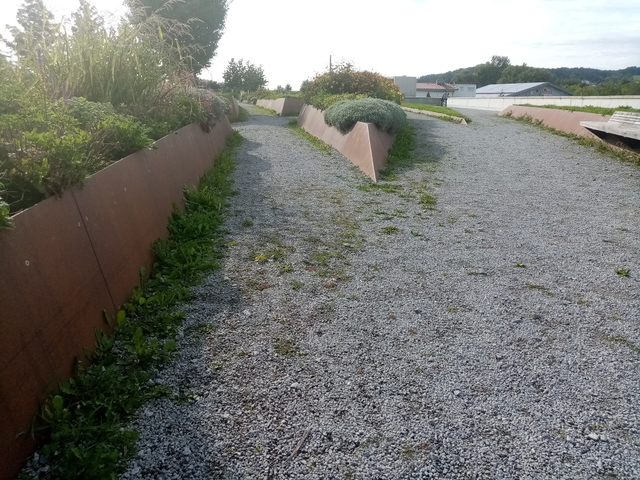
\includegraphics[width=0.48\textwidth]{images/deggendorf_example3.png}}
		\quad
		\subfloat[]{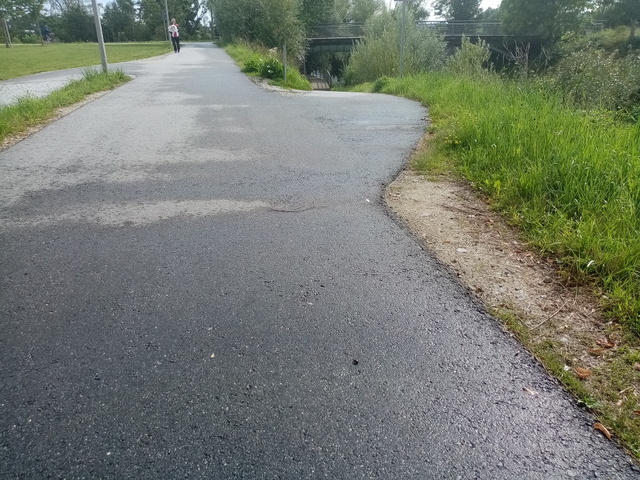
\includegraphics[width=0.48\textwidth]{images/deggendorf_example4.png}}
	\end{center}
	\caption[Examples from the city park of Deggendorf]{Examples from the city park of Deggendorf.}
	\label{img:deggendorf_examples}
\end{figure}

\section{Data preprocessing and augmentation}
\label{sec:data_augment}

In order to feed data to network one has to preprocess the image in some way.
Pictures produced by phone were in quite high resolution which would make the inference
time very high. We decided to scale them down to widely used resolution of
$640\times 480$ pixels. Labels in Lednice dataset contain $53.90\%$ of driveable segment
pixels and labels in Deggendorf dataset contain $61.14\%$ of driveable segment pixels.

Our images are in the \textbf{RGB} color space, which means that each one contains three channels
with values in range from 0 to 255. In order to make the model learn it is a common practice
to normalize these values so they are in range either from 0 to 1 or from -1 to 1. The former
can be reached by dividing all the channels by 255 and the latter by subtracting
mean and dividing by standard deviation per channel. Ground truth labels (masks) are just
2D matrices with binary values where \textbf{1} denotes driveable pixel and \textbf{0}
non-driveable one. Since these masks contain values 0 or 255 once loaded from disk,
we just divide them by 255 to get zeros and ones.

Image augmentation is essential when it comes to extending the dataset because of the need
for better generalization and preventing the model from overfitting.
From every image we generate several
augmented ones using \textit{imgaug} library \cite{bib:imgaug}.

\begin{itemize}
    \item \textbf{Rotation} - random rotation by 5 degrees
    \item \textbf{Horizontal Flip} - flip the image horizontally
    \item \textbf{Motion Blur} - the robot captures images while moving and they are
        often blurred. Motion Blur blurs images by random kernel $k=randint(3, 7)$
        to resemble real world scenario
    \item \textbf{Add Brightness} - add brightness by severity $s = 2$
    \item \textbf{Fog} - add fog to image
\end{itemize}

\textit{Rotation} and \textit{Horizontal Flip} transformations require the mask
to be augmented as well and thus we apply such transformation on mask.
Both augmented and original images are then being fed to ConvNet.

\section{Models and learning process}
\label{sec:learning}

\subsection{Losses}
\label{sec:learning:losses}

The \textit{loss} function (also called \textit{cost} or \textit{error} function) denotes
a function computing how bad is the model at predictions. The optimizer
updates model's weights to decrease the loss. Since we are not able to compute these
weights perfectly, training neural networks is an optimization problem where the loss 
function navigates us through the space of possible configurations.

There are many loss functions to choose from. The most common ones for semantic segmentation
used in literature are \textit{Binary crossentropy} and \textit{Dice coefficient loss}. 

\begin{itemize}
    \item \textbf{Binary crossentropy}
        $$\textrm{BCE}(y, \hat{y}) = -\frac{1}{N}\sum\limits_{i=1}^N y_i\cdot log(\hat{y_i}) + (1-y_i)\cdot log(1-\hat{y_i})$$
    \item \textbf{Dice coefficient loss}
        $$\textrm{DICE}(y, \hat{y}) = 1 - \frac{2\cdot y\cdot \hat{y} + \epsilon}{y + \hat{y} +
        \epsilon} =
        1 - \frac{2\cdot \sum\limits_{i=1}^N (y_i \cdot \hat{y_i}) +
        \epsilon}{\sum\limits_{i=1}^N y_i + \sum\limits_{i=1}^N \hat{y_i} + \epsilon}$$
\end{itemize}

The $N$ denotes the number of pixels,
$y_i$ denotes ground truth value for pixel at $i$-th position and $\hat{y_i}$ is the
output of the network at $i$-th position, which is interpreted as the probability of pixel
being driveable.

\subsection{Metrics}
\label{sec:learning:metrics}

Metrics are used to measure the performance of the model. Choosing the right metric
is a crucial part in order to compare models appropriately. We might sometimes also use loss
function as a metric, but in general a metric function does not have to be differentiable.
In our work, we are working with two most widely used metrics for segmentation task:

\begin{itemize}
    \item \textbf{Binary Accuracy}
        $$\textrm{ACC}(I) = \frac{TP + TN}{TP + TN + FP + FN}$$
    \item \textbf{Intersection over Union (IoU)}
        $$\textrm{IoU}(I) = \frac{1}{|I|}\sum\limits_{i=1}^{|I|}
        \frac{|Y_i\cap \hat{Y_i}|}{|Y_i\cup \hat{Y_i}|}$$
\end{itemize}

Since output of the network is in range between 0 and 1 for each pixel,
we need to round $\hat{Y}$ 
values. Threshold is set to $0.5$ meaning pixels with probability above $0.5$ get
classified driveable and conversely, pixels with probability below $0.5$ are classified
non-driveable. The argument $I$ is a set of images the metric is measured on.

The nominator in \textit{binary accuracy} metric represents the number of pixels
that are classified correctly, whilst denominator represents the total number of pixels
present across entire image set.

\textit{Intersection over Union} is measured as a mean of IoUs over the set $I$.
Simply put, it is the area of intersection between predicted segmentation mask and
ground truth divided by their union. IoU is the most popular metric in semantic
segmentation community sometimes referred to as \textit{Jaccard index}. 

Binary accuracy can sometimes provide misleading results and that's why
IoU is better in terms of correct overlaps. Now let's try to understand why this metric 
is better than binary accuracy. Imagine the model is asked to predict an image with
a small area of driveable segment. If the model classifies all the pixels as non-driveable
(returns mask filled with zeros) we get very high accuracy due to correct classification of
these zeros. However, the model's IoU is zero in this case which is desired result.

\section{Results}
\label{sec:first_results}

\subsection{HSV model}
\label{sec:first_results:hsv}

\begin{figure}[!h]
	\begin{center}
	    \subfloat[Trained on Lednice dataset]{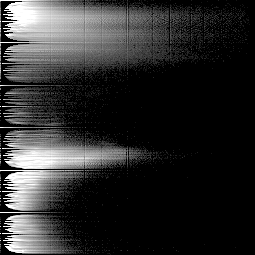
\includegraphics[width=0.48\textwidth]{images/hsv_positive_lednice.png}}
		\quad
		\subfloat[Trained on Deggendorf dataset]{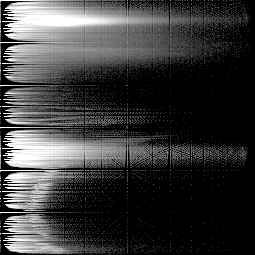
\includegraphics[width=0.48\textwidth]{images/hsv_positive_deggendorf.png}}
	\end{center}
	\caption[HSV model trained on Lednice and Deggendorf datasets]{HSV model trained on
	Lednice and Deggendorf datasets.
	\textit{Y} axis represents H values, \textit{X} axis represents S values
	and pixel intensity indicates how likely is the pixel driveable.}
	\label{img:hsv_positive}
\end{figure}

We took HSV model used on RoboTour 2018 and set it as our baseline. 

\begin{table}[h]
	\centering
	\begin{tabular}{|c||c|c|} 
		\hline
		dataset & test accuracy & test IoU \\
		\hline
		Lednice & 0.9037 & 0.8504 \\
		Deggendorf & 0.8006 & 0.7403 \\
		\hline
	\end{tabular}
	\caption[Results of HSV model measured on both datasets]{Results of HSV model measured on both datasets.}
	\label{tab:results_hsv_model}
\end{table}

Both datasets were split into \textit{train} and \textit{test} subsets. Training the
model produced matrices shown in Figure \ref{img:hsv_positive}.

According to pixel intensities we may notice higher uncertainty in Deggendorf dataset
which proves our assumption that this dataset is much more difficult to learn and predict.
There is a large number of pixels with same or almost the same color but classified
differently (i.e. grey pavement and grey wall).
Model's performance is captured in Table \ref{tab:results_hsv_model}. Although the Lednice
results might be acceptable, in case of Deggendorf the accuracy is not sufficient.


\subsection{KittiSeg}
\label{sec:kittiseg}

One of the decoders in MultiNet architecture \cite{bib:teichmann2018multinet}
is dedicated to semantic segmentation task. We wanted to test its performance on our Lednice
dataset in 2018 right before the competition in the Lednice park.

Encoders in this architecture were pretrained on ImageNet dataset \cite{bib:deng2009imagenet}
and we only wanted to fine-tune the model to our Lednice dataset. Since this architecture
is designed to perform binary semantic segmentation of driveable roads, it took
only few epochs to fine-tune it to city park. Results are captured in Table
\ref{tab:results_kittiseg}. The reason for not using it on robot is we were not able to
load it to Jetson's memory because of the model's huge size. NVIDIA Jetson TX2 GPU
mounted on our robot contains 8 GB of RAM, 256 NVIDIA CUDA cores and 6 CPU cores.

\begin{table}[h]
	\centering
	\begin{tabular}{|c||c|c|} 
		\hline
		type & train acc & val acc \\
		\hline
		no augmentation & 0.9571 & 0.9563 \\
		augmentation used & 0.9580 & \textbf{0.9566} \\
		\hline
	\end{tabular}
	\caption[Results of KittiSeg model training]{Results of KittiSeg model training on Lednice
	dataset.}
	\label{tab:results_kittiseg}
\end{table}

\subsection{ConvNet models}
\label{sec:first_results:convnets}

We decided to test four different models before RoboTour competition. Among many available
we picked these:
\begin{itemize}
    \item Unet
    \item SegNet
    \item ResNet with 16 identity blocks
    \item FCN VGG16 with 32x upsampling
\end{itemize}

The FCN model was not able to start learning, thus we discarded it from our experiments.
As long as we have had access
to external server with graphics processing unit (GPU) NVIDIA GeForce GTX 1080, training
procedure was far more efficient in terms of speed than on CPU.
Our experiments involve training the models on both datasets, testing both loss functions
and reporting pixel accuracy as well as intersection over union.

The environment we chose to work in is \textit{Python 3.6} which has support for many
useful tools necessary for computer vision and especially deep learning.
Furthermore, in order to work with neural network we decided to choose widely used \textit{TensorFlow} \cite{bib:tensorflow2015} framework.
On top of \textit{TensorFlow} backend we utilize \textit{Keras}
\cite{bib:chollet2015keras}. It is an open source library capable of running on top of
several backends. It focuses on being user-friendly by providing interfaces for higher
level abstractions and contains implementations for commonly used building blocks
in deep learning such as layers, optimizers, metrics, activation functions as well as
many utilities for manipulating data and evaluating models.

\begin{table}[h]
	\centering
	\begin{tabular}{|c||c|c|c|} 
		\hline
		model & disk size & \# params & prediction time on Jetson \\
		\hline
		ResNet & 33 MB & 2,753,729 & 0.24169 sec \\
		\hline
		SegNet & 60 MB & 7,818,117 & 0.36903 sec \\
		\hline
		Unet & 356 MB & 31,032,837 & 1.08655 sec \\
		\hline
	\end{tabular}
	\caption[Basic information about models]{Basic information about models. The size of the input image is $640\times 480$. The prediction time is computed as the average of 20 predictions.}
	\label{tab:results_model_sizes}
\end{table}

Table \ref{tab:results_led_degg} captures results of aforementioned models. These results
are split into two subtables in order to differentiate between Lednice
and Deggendorf dataset.

All the models were trained from scratch meaning all weights were randomly initialized.
We test both binary crossentropy and dice coefficient loss as well as both
\textit{RGB} and \textit{HSV} color spaces. We split both datasets into \textit{train},
\textit{validation} and \textit{test} subsets.
Deep learning models are usually
trained with some kind of \textit{early stopping condition} which prevents the model
from overfitting to training data and decreases the time needed for learning. In our case,
we set early stopping condition to monitor validation loss and stop the training process
when this loss does not decrease in 5\% of total epochs.

In Table \ref{tab:results_model_sizes} we report basic information about proposed models
and compare their average inference times on Jetson TX2 GPU.

When it comes to optimizing test intersection over union, binary crossentropy outperformed
dice coefficient
loss (but in general it does not have to be the case).
Furthermore, results indicate that models show better performance in RGB color space.
ResNet is almost always better than SegNet while having the lowest number of
parameters and the best inference time. Unet's disadvantage is its number of parameters
and undesirable inference time.
Evaluation of models shows that Lednice dataset
is easier to predict than Deggendorf dataset, like we observed with HSV baseline model.
An interesting fact is that we are often able to train these models in less than one hour
which makes it usable especially in competition setup where we sometimes need to retrain
model to specific conditions.

\begin{figure}[!h]
	\begin{center}
	    \subfloat[Before]{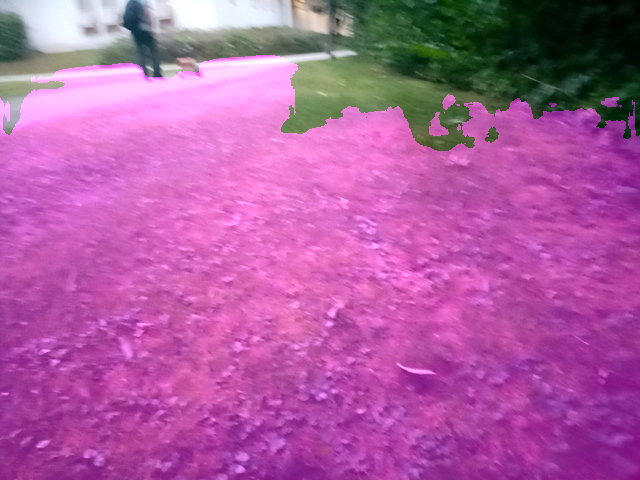
\includegraphics[width=0.48\textwidth]{images/bias_before.png}}
		\quad
		\subfloat[After]{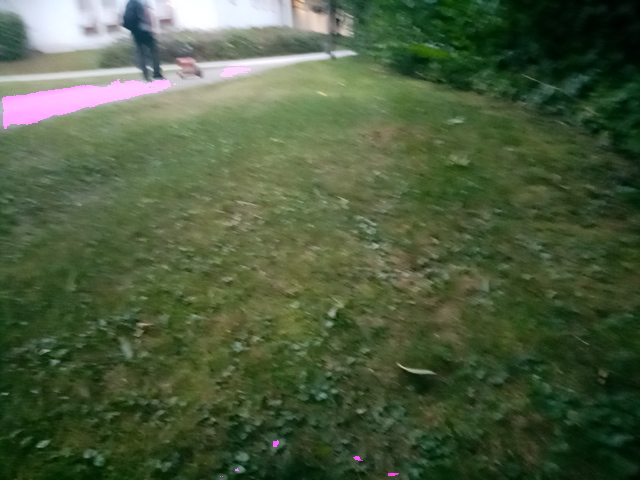
\includegraphics[width=0.48\textwidth]{images/bias_after.png}}
	\end{center}
	\caption[Predictions of images containing mostly grass]{Predictions of images containing mostly grass. Image (a) shows the prediction before this kind of images have been added to the dataset
	while image (b) is the prediction after the dataset has been extended. Both images
	are predicted by the same ResNet. The only thing that has changed is dataset.}
	\label{img:beforeafterextending}
\end{figure}


\subsubsection{AUC-ROC comparison}
\label{sec:first_results:convnets:aucroc}

\begin{figure}[h!]
	\begin{center}
	    \subfloat[Lednice dataset]{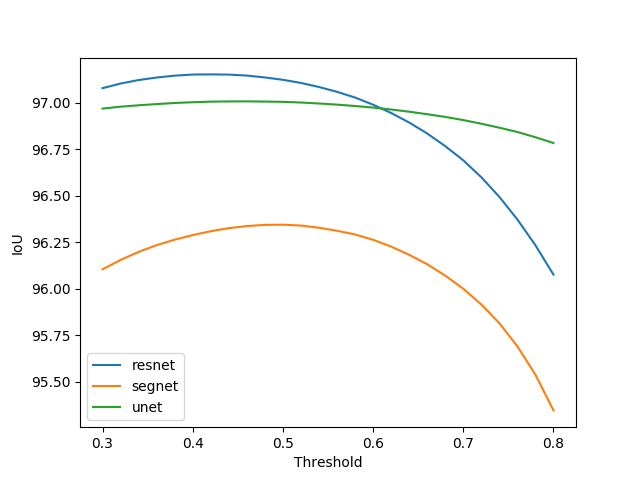
\includegraphics[width=0.49\textwidth]{images/lednice_thresholds_iou.png}}
	    \hspace{0.01em}
		\subfloat[Deggendorf dataset]{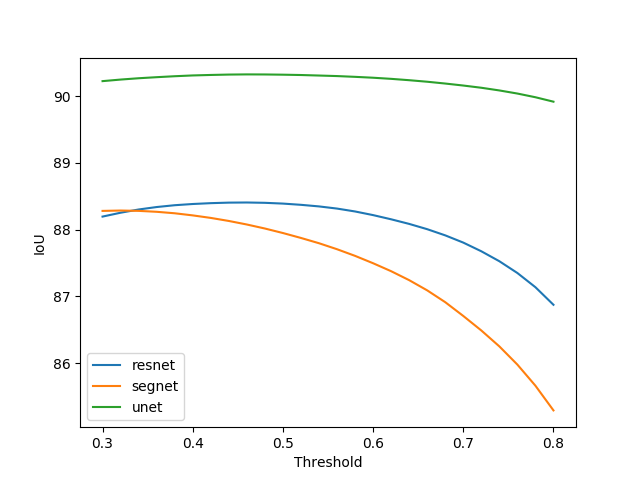
\includegraphics[width=0.49\textwidth]{images/deggendorf_thresholds_iou.png}}
	\end{center}
	\caption[Various rounding thresholds for ResNet, SegNet and Unet]{Comparison of various
	rounding thresholds for ResNet, SegNet and Unet (binary crossentropy loss with early
	stopping condition). The IoU is measured on test set.}
	\label{img:thresholds_base_models}
\end{figure}

Since the output from ConvNet is probability of each pixel being driveable, we need to define
threshold for rounding these probabilities to one and zero respectively. All the results
in Table \ref{tab:results_led_degg} were acquired using standard threshold of $0.5$, but
we also examined thresholds in range from $0.3$ to $0.8$.
According to Figure \ref{img:thresholds_base_models}, ResNet seems to work a little bit better
with thresholds close to $0.45$ on Deggendorf dataset whilst SegNet's best threshold values
are close to $0.3$. Interestingly, SegNet works better with threshold around $0.5$ on
Lednice dataset and Unet's accuracy stays almost unchanged on both datasets.
Once we noticed our models make mistakes on images covered mostly by non-driveable pixels
we extended Deggendorf dataset right before the competition which improved predictions
in production by huge margin, see Figure \ref{img:beforeafterextending}.

In order to select the best model which should be used in production,
a selection metric is chosen.
One of the most commonly used selection metrics is 
\textit{AUC-ROC} (Area Under Curve - Receiver Operating Characteristics) curve.
It is used to show performance of models at various threshold settings.
The plot consists of two parameters:
\begin{itemize}
    \item True Positive Rate denoted as $TPR = \frac{TP}{TP + FN}$
    \item False Positive Rate denoted as $FPT = \frac{FP}{FP + TN}$
\end{itemize}

\begin{figure}[h!]
	\begin{center}
	    \subfloat[Lednice dataset]{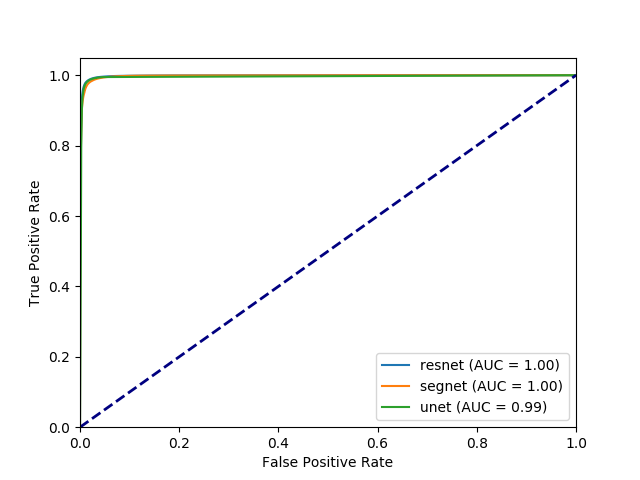
\includegraphics[width=0.49\textwidth]{images/lednice_roc.png}}
		\hspace{0.01em}
		\subfloat[Deggendorf dataset]{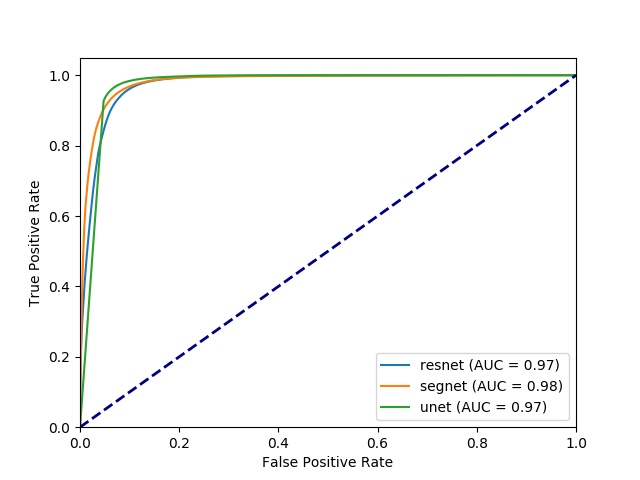
\includegraphics[width=0.49\textwidth]{images/deggendorf_roc.png}}
	\end{center}
	\caption[AUC - ROC comparison of ResNet, SegNet and Unet]{AUC - ROC comparison of ResNet,
	SegNet and Unet (binary crossentropy loss with early stopping condition).}
	\label{img:roc_base_models}
\end{figure}

In terms of the predicted probability, ROC tells us how good the model is
at distinguishing pixel's class.
Since AUC stands for Area Under Curve, it measures the entire two-dimensional area
under the ROC curve and provides an aggregate measure across all possible thresholds.
The bigger the area, the better the model is in distinguishing between driveable and
non-driveable pixels. If the AUC is equal to $0.5$, model's prediction are almost random with no
ability to distinguish between classes.

We compared our models using AUC-ROC curve. Figure \ref{img:thresholds_base_models} captures
these comparisons on both datasets. Their performance is very similar on Lednice dataset, but
SegNet works a bit better on Deggendorf dataset.
Since ResNet shows the best results overall (the best trade-off between test IoU and
inference time), we decided to use it at the competition in
Germany. During official runs predictions were quite good in terms of accuracy, but
the model's inference time is very high giving us only \textbf{four} frames per second (FPS).
This makes it very difficult for the robot to drive faster because it would suffer from
high latency between predictions. The visualization of test set predictions by ResNet and
SegNet is presented in Figure \ref{img:predictions_led_degg}.

\begin{figure}[!h]
	\begin{center}
	    \subfloat[Lednice]{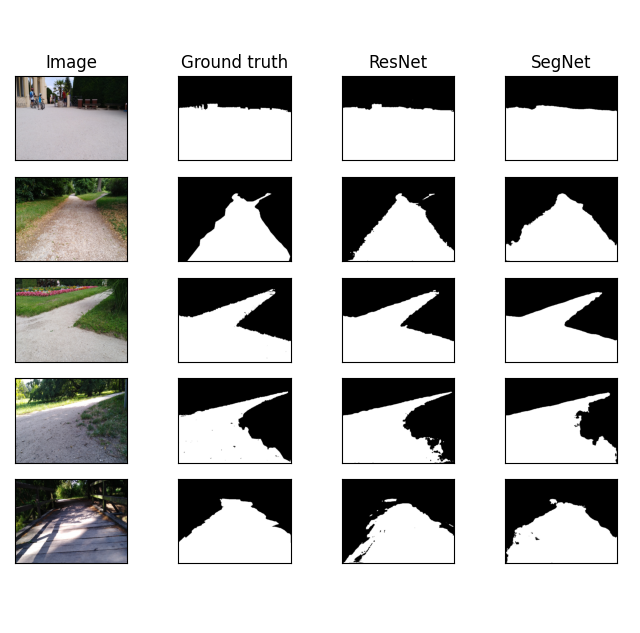
\includegraphics[width=0.49\textwidth]{images/lednice_predictions.png}}
		\hspace{0.01em}
		\subfloat[Deggendorf]{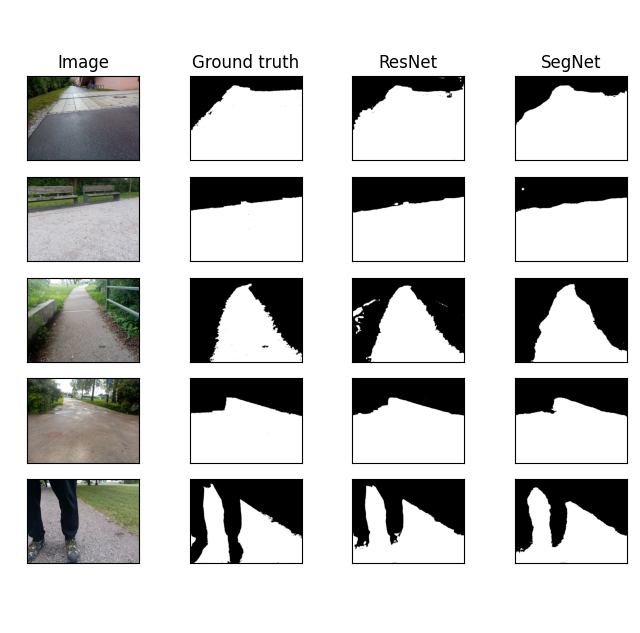
\includegraphics[width=0.49\textwidth]{images/deggendorf_predictions.png}}
	\end{center}
	\caption[Comparison of predictions against ground truths]{Comparison of test set predictions by ResNet and SegNet against ground truths.}
	\label{img:predictions_led_degg}
\end{figure}

\newpage
\begin{table}[h!]
	\centering
	\begin{tabular}{|c||c|c|c|c|c|c|c|c|} 
		\hline
		model & clr & loss & time & eps & train acc & train IoU & test acc & test IoU \\
		\hline
		ResNet & rgb & dcl & 81m & 77 & 0.9847 & 0.9673 & 0.9840 & 0.9700 \\
		SegNet & rgb & dcl & 191m & 167 & 0.9808 & 0.9578 & 0.9709 & 0.9484 \\
		Unet & rgb & dcl & 523m & 157 & 0.9925 & 0.9842 & 0.9846 & \textbf{0.9715} \\
		ResNet & rgb & bce & 76m & 70 & 0.9867 & 0.9698 & 0.9845 & 0.9711 \\
        SegNet & rgb & bce & 114m & 100 & 0.9845 & 0.9649 & 0.9809 & 0.9643 \\
        Unet & rgb & bce & 434m & 130 & 0.9948 & 0.9888 & 0.9841 & 0.9705\\
        \hline
        ResNet & hsv & dcl & 45m & 42 & 0.9758 & 0.9496 & 0.9815 & 0.9660 \\
        SegNet & hsv & dcl & 144m & 125 & 0.9769 & 0.9493 & 0.9756 & 0.9562 \\
        ResNet & hsv & bce & 54m & 50 & 0.9818 & 0.9594 & 0.9853 & \textbf{0.9725} \\
        SegNet & hsv & bce & 52m & 45 & 0.9768 & 0.9487 & 0.9751 & 0.9554 \\
        \hline
        ResNet & rgb & dcl & 155m & 150 & 0.9848 & 0.9680 & 0.9828 & 0.9683 \\
        SegNet & rgb & dcl & 171m & 150 & 0.9796 & 0.9552 & 0.9767 & 0.9580 \\
        ResNet & rgb & bce & 159m & 150 & 0.9823 & 0.9604 & 0.9839 & \textbf{0.9694} \\
        SegNet & rgb & bce & 172m & 150 & 0.9854 & 0.9668 & 0.9790 & 0.9619 \\
		\hline
	\end{tabular}

	\bigskip

    \begin{tabular}{|c||c|c|c|c|c|c|c|c|} 
		\hline
		model & clr & loss & time & eps & train acc & train IoU & test acc & test IoU \\
		\hline
		ResNet & rgb & dcl & 44m & 40 & 0.9605 & 0.9259 & 0.9378 & 0.8878 \\
		SegNet & rgb & dcl & 122m & 104 & 0.9660 & 0.9302 & 0.9222 & 0.8551 \\
		Unet & rgb & dcl & 499m & 145 & 0.9834 & 0.9606 & 0.9506 & 0.9017 \\
		ResNet & rgb & bce & 42m & 38 & 0.9625 & 0.9269 & 0.9366 & 0.8838 \\
        SegNet & rgb & bce & 57m & 48 & 0.9671 & 0.9357 & 0.9403 & 0.8795 \\
        Unet & rgb & bce & 451m & 131 & 0.9908 & 0.9715 & 0.9521 & \textbf{0.9031} \\
        \hline
        ResNet & hsv & dcl & 61m & 55 & 0.9546 & 0.9165 & 0.9376 & \textbf{0.8868} \\
        SegNet & hsv & dcl & 192m & 167 & 0.9656 & 0.9303 & 0.9329 & 0.8788 \\
        ResNet & hsv & bce & 86m & 75 & 0.9750 & 0.9410 & 0.9409 & 0.8861 \\
        SegNet & hsv & bce & 97m & 81 & 0.9738 & 0.9415 & 0.9308 & 0.8748 \\
        \hline
        ResNet & rgb & dcl & 160m & 150 & 0.9784 & 0.9504 & 0.9445 & 0.8953 \\
        SegNet & rgb & dcl & 176m & 150 & 0.9687 & 0.9357 & 0.9189 & 0.8494 \\
        ResNet & rgb & bce & 164m & 150 & 0.9766 & 0.9459 & 0.9491 & \textbf{0.8958} \\
        SegNet & rgb & bce & 177m & 150 & 0.9784 & 0.9486 & 0.9386 & 0.8793 \\
		\hline
	\end{tabular}

	\caption[Results of various models trained on Lednice and Deggendorf datasets]{Results -
	the first table describes results on \textbf{Lednice} dataset and
	the second table on \textbf{Deggendorf} dataset.
	Models in last four rows in both tables were trained for 150 epochs,
	whilst the other ones used early stopping condition monitoring validation loss.
	Dice coefficient loss is marked as \textit{dcl} and binary crossentropy as \textit{bce}.
	\textit{Clr} denotes color space of images, \textit{time} is training time and  
	\textit{eps} is the number of epochs.}
	\label{tab:results_led_degg}
\end{table}

\newpage

\subsection{Testing models on unseen dataset}
\label{sec:first_results:oppositedataset}

Imagine the robot is participating at the competition in environment we do not have dataset
from. Since obtaining a new dataset along with labeling all of its images is very time
consuming we cannot afford to prepare the model in such a short period of time.
Thus, we want to train our models on other dataset (obtained at previous contests)
and use it in a new environment. This approach is often reffered to as transfer learning.

Table \ref{tab:opposite_datasets} shows performance of models described in Section
\ref{sec:first_results:convnets} on unseen datasets.

Surprisingly, if we compare these results with Table \ref{tab:results_led_degg},
we can clearly see that there is not a big difference in terms of accuracy and
models perform relatively well on unseen datasets. The IoU is worse by 3\% on average, but
the IoU is high enough for predicting driveable path
and therefore we can conclude that models trained on specific dataset may be used in
a similar environment.

\begin{table}[!h]
	\centering
	\subfloat[Lednice models on Deggendorf dataset]{
    	\begin{tabular}{|c||c|c|c|c|}
    	    \hline
    		model & clr & loss & acc & iou \\
    		\hline
    		ResNet & rgb & dcl & 0.9144 & 0.8475 \\
    		SegNet & rgb & dcl & 0.9157 & 0.8502 \\
    		Unet & rgb & dcl & 0.9360 & 0.8810 \\
    		ResNet & rgb & bce & 0.9036 & 0.8278 \\
            SegNet & rgb & bce & 0.9146 & 0.8439 \\
            Unet & rgb & bce & 0.9357 & \textbf{0.8812} \\
            \hline
            ResNet & hsv & dcl & 0.8939 & 0.8189 \\
            SegNet & hsv & dcl & 0.8893 & 0.8171 \\
            ResNet & hsv & bce & 0.8887 & 0.8110 \\
            SegNet & hsv & bce & 0.8835 & 0.8003 \\
            \hline
            ResNet & rgb & dcl & 0.9230 & \textbf{0.8616} \\
            SegNet & rgb & dcl & 0.9103 & 0.8383 \\
            ResNet & rgb & bce & 0.9192 & 0.8509 \\
            SegNet & rgb & bce & 0.9093 & 0.8351 \\
            \hline
    	\end{tabular}
    }
    \hspace{0.5em}
    \subfloat[Deggendorf models on Lednice dataset]{
    	\begin{tabular}{|c||c|c|c|c|}
    	    \hline
    		model & clr & loss & acc & iou \\
    		\hline
    		ResNet & rgb & dcl & 0.9624 & 0.9289 \\
    		SegNet & rgb & dcl & 0.9563 & 0.9149 \\
    		Unet & rgb & dcl & 0.9654 & 0.9324 \\
    		ResNet & rgb & bce & 0.9626 & 0.9271 \\
            SegNet & rgb & bce & 0.9597 & 0.9206 \\
            Unet & rgb & bce & 0.9689 & \textbf{0.9382} \\
            \hline
            ResNet & hsv & dcl & 0.9637 & \textbf{0.9300} \\
            SegNet & hsv & dcl & 0.9532 & 0.9108 \\
            ResNet & hsv & bce & 0.9617 & 0.9242 \\
            SegNet & hsv & bce & 0.9526 & 0.9074 \\
            \hline
            ResNet & rgb & dcl & 0.9644 & 0.9312 \\
            SegNet & rgb & dcl & 0.9535 & 0.9103 \\
            ResNet & rgb & bce & 0.9656 & \textbf{0.9323} \\
            SegNet & rgb & bce & 0.9583 & 0.9199 \\
            \hline
    	\end{tabular}
    }
    \caption[Results of models tested on unseen dataset]{Results of models tested on full unseen dataset}
    \label{tab:opposite_datasets}
\end{table}
